% This file was created with tikzplotlib v0.9.17.
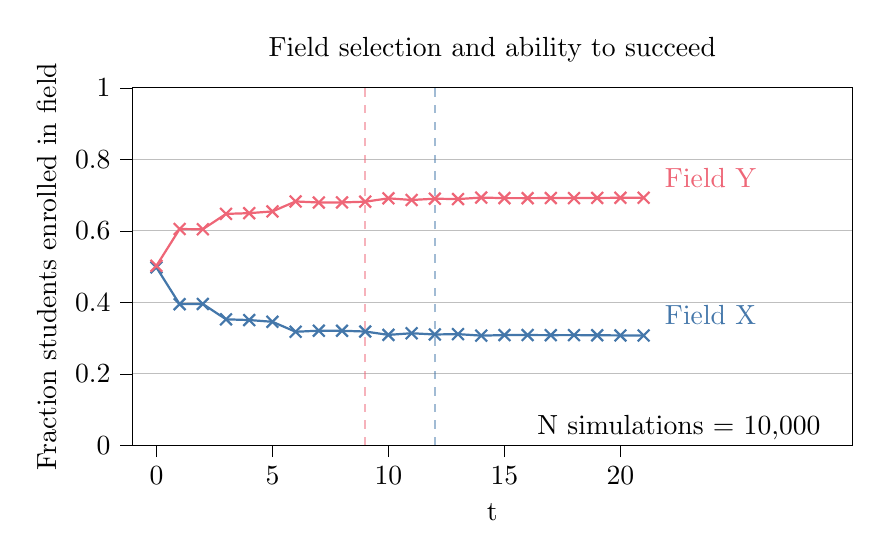
\begin{tikzpicture}

\definecolor{color0}{rgb}{0.266666666666667,0.466666666666667,0.666666666666667}
\definecolor{color1}{rgb}{0.933333333333333,0.4,0.466666666666667}

\begin{axis}[
height=6.121302808757603cm,
tick align=outside,
tick pos=left,
title={Field selection and ability to succeed},
width=10.729849cm,
x grid style={white!69.0196078431373!black},
xlabel={t},
xmin=-1.05, xmax=30,
xtick style={color=black},
xtick={0,5,10,15,20},
xticklabels={
  \(\displaystyle 0\),
  \(\displaystyle 5\),
  \(\displaystyle 10\),
  \(\displaystyle 15\),
  \(\displaystyle 20\)
},
ylabel={Fraction students enrolled in field},
ymajorgrids,
ymin=0, ymax=1,
ytick style={color=black},
ytick={0,0.2,0.4,0.6,0.8,1},
yticklabels={
  \(\displaystyle 0\),
  \(\displaystyle 0.2\),
  \(\displaystyle 0.4\),
  \(\displaystyle 0.6\),
  \(\displaystyle 0.8\),
  \(\displaystyle 1\)
}
]
\addplot [thick, color0, mark=x, mark size=3, mark options={solid}]
table {%
0 0.4977
1 0.3949
2 0.3955
3 0.3525
4 0.3505
5 0.3456
6 0.3177
7 0.3207
8 0.3205
9 0.3184
10 0.309
11 0.3136
12 0.3101
13 0.3111
14 0.3069
15 0.3084
16 0.3085
17 0.3082
18 0.3084
19 0.3079
20 0.3075
21 0.3074
};
\addplot [thick, color1, mark=x, mark size=3, mark options={solid}]
table {%
0 0.5023
1 0.6051
2 0.6045
3 0.6475
4 0.6495
5 0.6544
6 0.6823
7 0.6793
8 0.6795
9 0.6816
10 0.691
11 0.6864
12 0.6899
13 0.6889
14 0.6931
15 0.6916
16 0.6915
17 0.6918
18 0.6916
19 0.6921
20 0.6925
21 0.6926
};
\addplot [semithick, color0, opacity=0.5, dashed]
table {%
12 0
12 1
};
\addplot [semithick, color1, opacity=0.5, dashed]
table {%
9 0
9 1
};
\draw (axis cs:21.5,0.3374) node[
  anchor=base west,
  text=color0,
  rotate=0.0
]{Field X};
\draw (axis cs:21.5,0.7226) node[
  anchor=base west,
  text=color1,
  rotate=0.0
]{Field Y};
\draw (axis cs:16,0.03) node[
  anchor=base west,
  text=black,
  rotate=0.0
]{N simulations = 10,000};
\end{axis}

\end{tikzpicture}
